% !TeX root = ../ecuaciones-diferenciales.tex

\chapter{Introducci\'{o}n a las ecuaciones diferenciales}

\section{Idea intuitiva}
\begin{dfn}[Ecuacion diferencial de primer orden]
	Sea $\mbf{y} = f(x)$, una \textbf{ecuación diferencial de primer orden} es una ecuación de la forma: $\mbf{y'}=F(x,\mathbf{y})$.\\
    Sea $g(x)$ una función de x, diremos que es solución cuando la ecuación diferencial se cumpla para $\mbf{y} = g(x)$.
\end{dfn}

Veamos unos ejemplos típicos.

\begin{eg}
    Consideramos $\P \equiv x'(t) = 2x(t)$ (o alternativamente $\mbf{x}' = 2\mbf{x}$)\\
    Vemos que es una ecuación diferencial de primer orden ya que sigue la definición anterior. Es sencillo ver que $F(t,\mbf{x}) = 2\mbf{x} = 2x(t)$. Queremos hallar que funciones resuelven $P$\\
    Además, observamos que si $x(t) = e^{2t}$, entonces $x'(t) = 2e^{2t} = 2x(t)$ y por tanto $x(t) = e^{2t}$ es una solución de $P$.\\Si pensamos con más cuidado también observamos que $x(t) = 7e^{2t}$ también satisface $P$.\\
    Nos interesaría entonces hallar una \textbf{solución general}, que con una sola ecuación englobe todas las soluciones. Aunque de momento no podemos justificarlo, si tomamos $x(t) = ae^{2t} \mid a \in \R$ entonces se cumple que $x'(t) = 2ae^{2t} = 2x(t)$ y por tanto es la solución general de $P$.
\end{eg}

Del ejemplo anterior surgen problemas llamados \textit{problema de valor inicial}, donde hallando la solución general y sabiendo la imagen de un punto $t_0$ por medio de $x(t)$ podemos determinar el parámetro y encontrar una solución explícitamente. Como continuación al ejemplo anterior consideremos el sistema:
$$
    \begin{cases}
        x'(t) = 2x(t) \\ x(0) = 8
    \end{cases}
$$
Para resolverlo, hallamos la solución general $x(t) = ae^{2t}$ y sustituimos la segunda ecuación. $x(0) = ae^{0} = 8 \implies a = 8$.

\begin{eg}
    Consideramos $\P \equiv x'(t) = 3(x(t))^{\sfrac{2}{3}}.$, queremos hallar \textit{la} solución para $x(0)=0$.\\
    Empezamos hallando soluciones a la ecuación, en este caso $x(t) = t^3$ y $x(t) = 0$ resuelven la ecuación. Nuestro sistema sería:
    $$
        \begin{cases}
            x'(t) = 3(x(t))^{\sfrac{2}{3}} \\ x(0) = 0
        \end{cases}
    $$
    Sin embargo, tanto $x(t) = t^3 \mid t = 0$ como $x(t) = 0$ resuelven $P$. No podemos hablar de \textit{la} solución puesto que hay dos.
\end{eg}

En los dos ejemplos anteriores tenemos una ecuación diferencial de la forma $\mbf{x'} = F(t, \mbf{x})$, $f(\mbf{x}) = 2\mbf{x}$ y $f(\mbf{x}) = 3\mbf{x}^{\sfrac{2}{3}}$ respectivamente. Sin embargo, en la segunda tenemos dos soluciones para $x(0) = 0$. Al observar las gráficas de las dos funciones se ve la razón a simple vista, la segunda no es derivable en $0$.
\begin{center}
    \begin{tikzpicture}
        \begin{axis}[domain=-5:5,samples=150,
        restrict y to domain=-10:10,
        xtick=\empty,ytick=\empty,
        %extra x ticks={0.8,1.4}, linea vertical
        %extra y ticks=3.333333,extra y tick labels={$\frac{10}{3}$}, linea horizontal
        grid=both,axis lines=middle
        ]
            \addplot+[no marks, thick] ({x},{2*x}) node[pos=0.3, below, sloped] {$f(x)=2x$};
            \addplot+[no marks, black, thick,samples=400] ({x},{3*x^(2/3)}) node[near end, below, sloped] {$f(x)=3x^{\sfrac{2}{3}}$};
            \addplot+[no marks, black, thick,samples=400] ({-x},{3*x^(2/3)});
        \end{axis}
    \end{tikzpicture}
\end{center}

\begin{eg}[Crecimiento de una población]
    Consideramos $\P \equiv \mbf{x'} = \lambda \mbf{x}$. ($\lambda$ típicamente es natalidad o mortalidad).\\
    Sabiendo que modela el crecimiento de una población en función del tiempo, podemos aproximar (veremos por qué más adelante)
    $\frac{\Delta x}{\Delta t} \sim \dd{x}{t} = \mbf{x'}$. Por tanto (como $\lamda$ es una tasa, se entiende que el tiempo tiende a 0 para hallarla):
    $$ \frac{\Delta x}{\Delta t}\sim \dd{x}{t} = \lambda \cdot \mbf{x} \implies \lambda = \lim_{t \to 0} \frac{\mbf{x'}}{\mbf{x}}$$.
\end{eg}

El crecimiento de una población de organismos lo suficientemente grandes no se ve representada por la ecuación anterior debido a la limitación de recursos. Interesaría por tanto modelizar la ecuación teniendo esto en cuenta. Para ello utilizaremos el parámetro $L$ como el límite al que tendería la población con los recursos existentes.

\begin{eg}[Crecimiento de una población con limitación de recursos]
    Consideramos $\P \equiv \mbf{x'} = a(1-\frac{\mbf{x}}{L})\mbf{x}$ con $a > 0$. De esta forma cuando $\mbf{x} << L$ o $\mbf{x} >> L$ , tenemos prácticamente la ecuación del ejemplo anterior. Si $\mbf{x} \sim L$ entonces la población apenas crece/decrece. Para encontrar soluciones a esta ecuación no hace falta resoverla, basta graficarla. Partimos de $\mbf{x'} = f(t, \mbf{x}) = a (1 - \frac{\mbf{x}}{L})\mbf{x}$.
    \\
    \begin{center}
        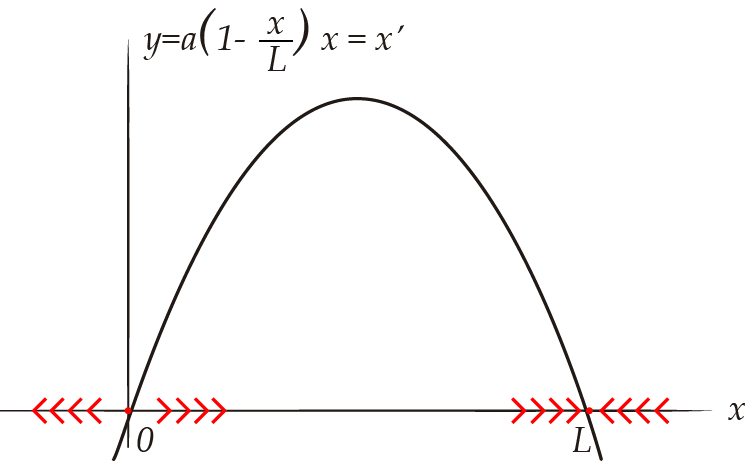
\includegraphics{1-limiterecursos.png}\label{img:1-limiterecursos}
    \end{center}
    Es fácil ver que $\mbf{x'}$ es una parábola, que corta al eje X en $0$ y $L$. Además, se indica con (>>) la dirección en la que se mueve $x(t)$ conforme avanza $t$. Tanto $0$ como $L$ son puntos de equilibrio, repulsor (inestable) y atractor (estable) respectivamente.
\end{eg}
\break

\begin{wrapfigure}{r}{0.5\textwidth}
  \begin{center}
    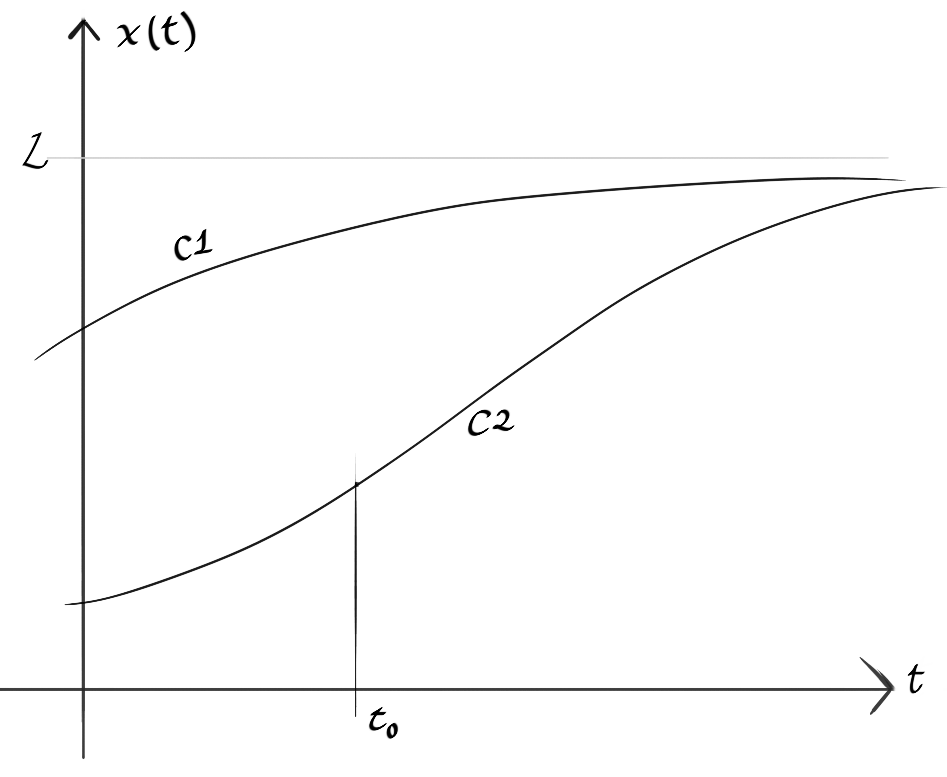
\includegraphics[width=0.48\textwidth]{1-poblaciontiempo.png}
  \end{center}
  \caption{Población - Tiempo}\label{img:1-poblaciontiempo}
\end{wrapfigure}
Habiendo encontrado las soluciones de la funcion anterior, nos preguntamos como varía la población frente al tiempo. Más adelante veremos formalmente como representar $\mbf{x}$ frente a $t$. Sin embargo, podemos razonar el aspecto de la función.
Sabemos que tiene que corregirse cerca de L, y que si $\mbf{x} << L$ entonces tiene un crecimiento parecido al exponencial. Por tanto, podría tener el aspecto de la figura \ref{img:1-poblaciontiempo}.
De este gráfico podemos deducir varias cosas. Para empezar, sabemos que $\mbf{x''}(t_0)=0$ tiene solución para la curva $c_2$ ya que tiene un punto de inflexión. Además, observamos disintos tipos de crecimiento en función del valor de $x(0)$ por lo que tendría sentido intentar determinar para qué valores $x_0$ obtenemos el crecimiento de $c_1$ y para cuáles el de $c_2$.

\begin{th_ex}\label{thex:29/01-0}
    ¿Para qué valores de $x_0$ se dan los diferentes crecimientos de $c_1$ y $c_2$?.\\
    \textit{Sugerencia}: Considerar el problema de valor inicial con $x''(t_0) = 0$.
\end{th_ex}

\section{Método de separación de variables}
Esta sección trata sobre el primer método de resolución de ecuaciones diferenciales. Antes de definir el método formalmente vamos a ver un ejemplo.
\begin{eg}[Resolución sencilla]
    Sea $\P \equiv \mbf{y'} = x\mbf{y}$. Halla las soluciones de la ecuación.\\
    $\mbf{y'} = \dd{y}{x}$, con esta igualdad podemos hacer manipulaciones sin justificar (de momento).
    $$
        \dd{y}{x} = x \mbf{y} \implies \frac{dy}{\mbf{y}} = x\mathrm{d}x \implies \int \frac{dy}{\mbf{y}} = \int x\mathrm{d}x \implies \log|\mbf{y}| = \frac{x^2}{2} + C \implies |\mbf{y}| = e^{\sfrac{x^2}{2} + C} = e^C \cdot e^{\sfrac{x^2}{2}}
    $$
    $$
        \mbf{y} = \pm e^C \cdot e^{\sfrac{x^2}{2}} = ke^{\sfrac{x^2}{2}} \mid k \in \R
    $$
\end{eg}
Esta resolución se conoce como método de separación de variables.
\begin{th_ex}\label{thex:29/01-1}
    Resolver $\P \equiv \mbf{x'} = a(1-\sfrac{\mbf{x}}{L})\mbf{x}$ con $x(0)=0$.\\
\end{th_ex}
Vamos a generalizar el método por medio de la siguiente proposición.
\begin{pro}[Método de separación de variables]
    Sea $F(x)$ una primitiva de $f(x)$ y $G(\mbf{y})$ una primitiva de $g(\mbf{y})$, es decir, $\dd{F}{x} = f(x)$ y $\dd{G}{\mbf{y}} = g(\mbf{y})$, con $\mbf{y} = f(x)$. Y sea una ecuación $\P \equiv \dd{y}{x} = \frac{f(x)}{g(\mbf{y})}$, entonces las soluciones de $\P$ cumplen:
    $$
        G(y(x)) = F(x) + \mathcal{C} \mid \mathcal{C}\ constante.
    $$
\end{pro}

\begin{proof}
    \begin{align*}
        \intertext{Por la regla de la cadena:}
            &\Dd{x} G(y(x)) = \dd{G}{\mbf{y}}(y(x)) \cdot \dd{y}{x}(x) \\
        \intertext{Como $\dd{G}{\mbf{y}} = g(\mbf{y})$ y $\dd{y}{x} = \frac{f(x)}{g(\mbf{y})}$   por hipóstesis:}
            &\dd{G}{\mbf{y}}(y(x)) \cdot \dd{y}{x}(x) = g(y(x)) \cdot \frac{f(x)}{g(y(x))} = f(x) = \Dd{x} F(x)
        \intertext{Es decir:}
            &\Dd{x}G(y(x)) = \Dd{x}F(x) \implies \Dd{x}G(y(x)) - \Dd{x}F(x) = 0 \implies G(y(x)) - F(x)  =  \mathcal{C} \implies G(y(x)) = F(x) + \mathcal{C}
    \end{align*}
\end{proof}
\begin{obs}
    La prosposición anterior está incompleta, faltaría ver que condiciones tienen que cumplir $f(x)$ y $g(\mbf{y})$. Para completarla tenemos que considerar la existencia de primitivas y la condición de que $\mathcal{C}$ sea constante.
    \begin{itemize}
        \item Ya que tenemos que usar que $F(x)$ y $G(\mbf{y})$ son primitivas, basta pedir que tanto $f(x)$ y $g(\mbf{y})$ sean continuas. Esto garantiza que $F(x)$ y $G(\mbf{y})$ son ambas $C^1$
        \item Si $h'(x) = 0 \implies h(x)$ constante en cada intervalo en que está definida (pues $\R$ es conexo). Si $h:\R \rightarrow \R$ entonces $h(x)$ es constante. Como $\mathcal{C}$ surge de integrar $0$ a la derecha de la ecuación, podemos afirmar que $\mathcal{C} = h(x)$ y por tanto constante.
    \end{itemize}
\end{obs}
\section{Significado geométrico de la ecuación diferencial ordinaria}
Vamos a analizar una ecuación diferencial de forma gráfica para interpretarla geométricamente. Consideramos $\mbf{y'} = f(x, \mbf(y))$. Supongamos que $\mbf{y}$ tiene la gráfica de la figura \ref{img:1-siggeom}.
\begin{figure}[h]
\begin{subfigure}{.5\textwidth}
    \centering
    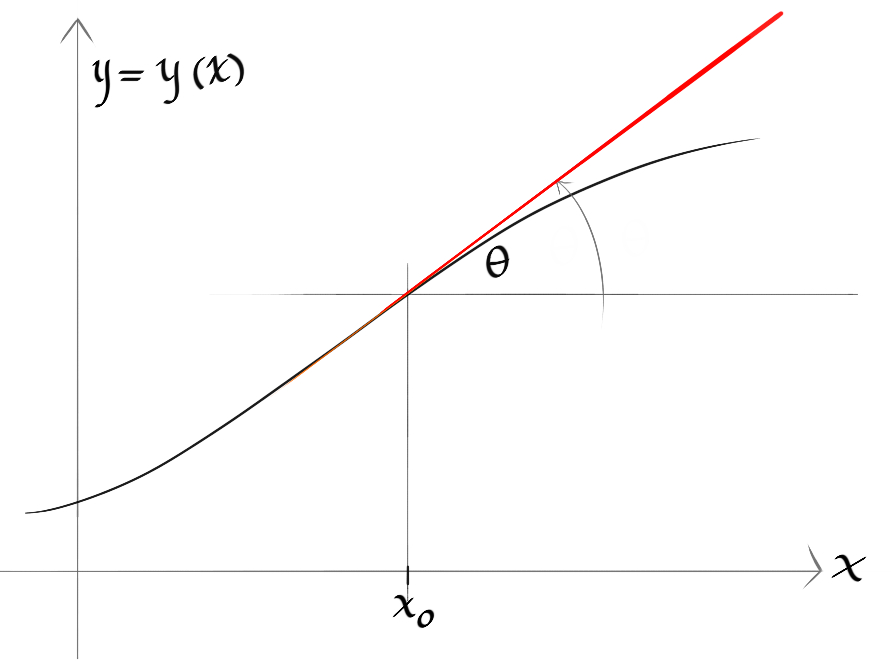
\includegraphics[width=1\textwidth]{1-significadogeom.png}
    \caption{Recta tangente en $x_0$ conocidas $\mbf{y}$ y $x_0$}\label{img:1-siggeom}
\end{subfigure}
\begin{subfigure}{.5\textwidth}
    \centering
    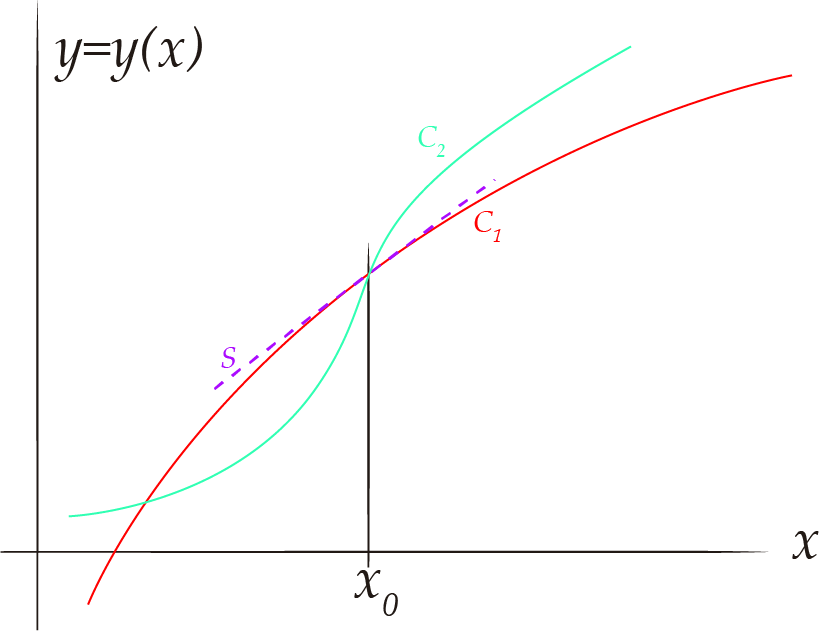
\includegraphics[width=1\textwidth]{1-significadogeom2.png}
    \caption{Curvas dadas el segmento $\mathcal{S}$.}\label{img:1-siggeom2}
\end{subfigure}
\end{figure}
Entonces, $\mbf{y'}(x_0) = \tan{\theta}$, que es la pendiente de la recta tangente a la gráfica de $\mbf{y}$ en $x_0$. Esto es cálculo elemental, lo que nos interesa es saber algo de la función $\mbf{y}$ cuando sabemos algo de $\mbf{y'}$.\\

Ilustramos en la figura \ref{img:1-siggeom2} entonces la casuística de conocer $\P \equiv \mbf{y'} = f(x,\mbf{y})$. En este caso, nos preguntamos que aspecto podría tener $\mbf{y}$ para que fuera solución de $\P$. Como conocemos $y'(x_0)$, podemos considerar que $\mathcal{S}$ es un semento paralelo a la recta tangente de la gráfica en $x_0$. Es fácil ver que $\mathcal{C}_1$ no puede ser solución de $\P$ pues $\mathcal{C}'_1(x_0) \neq y'(x_0)$. Sin embargo, es evidente que $\mathcal{C}_2$ sí resuelve $\P$.\\\\
Si repetimos el procedimiento de determinar como son las pendientes (como acabamos de hacer para $x_0$) para todos los puntos, hallamos el \textit{campo de pendientes}.

\begin{eg}[Hallar un campo de pendientes]
    Sea $\P \equiv \mbf{x'} = t^2 + \mbf{x}^2$, es decir, $f(t, \mbf{x}) = t^2 + \mbf{x}^2$. Si queremos hallar qué pendiente se le asigna al punto $p = (\sfrac{1}{\sqrt{2}},\sfrac{1}{\sqrt{2}})$ evaluamos la función $f$, $f(p) = 1$. Por tanto, la función $\mbf{x}$ que soluciona $\P$ tiene tangente con pendiente $1$ en $t = \sfrac{1}{\sqrt{2}}$.\\\\
    De hecho, es lógico pensar que a cualquier punto que cumpla $t^2 + \mbf{x}^2 = 1$ se le asignará una pendiente de $1$ a su recta tangente. Este conjunto de puntos conforman la \textbf{isoclina} de pendiente 1.\\\\
    De forma general, para una constante $c$ dada (en este ejemplo necesariamente no negativa pues $f(t, \mbf{x})$ es suma de cuadrados), podemos definir la isoclina de pendiente c:
    $$
    ISO_c = \left\{(t, \mbf{x}) \mid f(t, \mbf{x}) = c\right\}
    $$
    Volviendo a nuestro ejemplo, las isoclinas van a ser curvas que cumplan $t^2 + \mbf{x}^2 = c$ para un $c$ dado.\\
    \begin{minipage}[c]{0.3\linewidth}
      \begin{center}
          \raisebox{\dimexpr \topskip-\height}{
        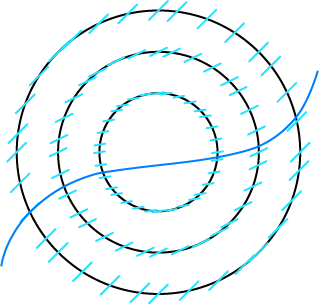
\includegraphics[width=\textwidth]{1-isoclinas.png}}
      \end{center}
    \end{minipage}\hfill
    \begin{minipage}[c]{0.65\textwidth}
        Hemos representado las isoclinas junto con un pequeño segmento de pendiente $c$ para disintos valores de $c$. Como las isoclinas cumplen que $t^2 + \mbf{x}^2 = c$, estas son las circumferencias de radio $\sqrt{c}$ con $c > 0$.\\
        Podemos observar tambien que $ISO_0 = \{(0,0)\}$ e $ISO_{c < 0} = \varnothing$.\\\\ Llamamos a la gráfica con pequeños segmentos \textit{campo de pendientes} y por tanto, una función que resuelva $\P$ tiene que ser tangente al segmento del punto por el que pase.
    \end{minipage}
    Sin embargo, los campos de pendientes permiten ver cómo es la función a grandes rasgos. En nuestro ejemplo parece indicar que $x(t) \uparrow \infty$, pero no sabemos si lo hace de forma asintótica ($x(t) \uparrow \infty$ en t finito), o x(t) crece a infinito cuando $t \rightarrow \infty$.\\
    Esto no puede resolverse gráficamente y veremos como resolverlo de forma analítica más adelante.
\end{eg}

\section{Ecuaciones diferenciales y problemas geométricos}
Gracias a la relación de la derivada con la tangencia de funciones, podemos plantear problemas geométricos en forma de ecuación diferencial.
\subsection{Trayectorias ortogonales}
De la recta tagente a un punto surge el concepto de recta normal a ese punto, que no es más que la recta perpendicular a la tangente y que pasa por dicho punto. Para ver como se relacionan estas dos rectas vamos a hacer un análisis simple. Diremos que dos curvas son ortogonales si en el punto de cruce las rectas tangentes a cada curva son perpendiculares entre sí.
\begin{wrapfigure}[20]{l}{0.5\textwidth}
  \begin{center}
    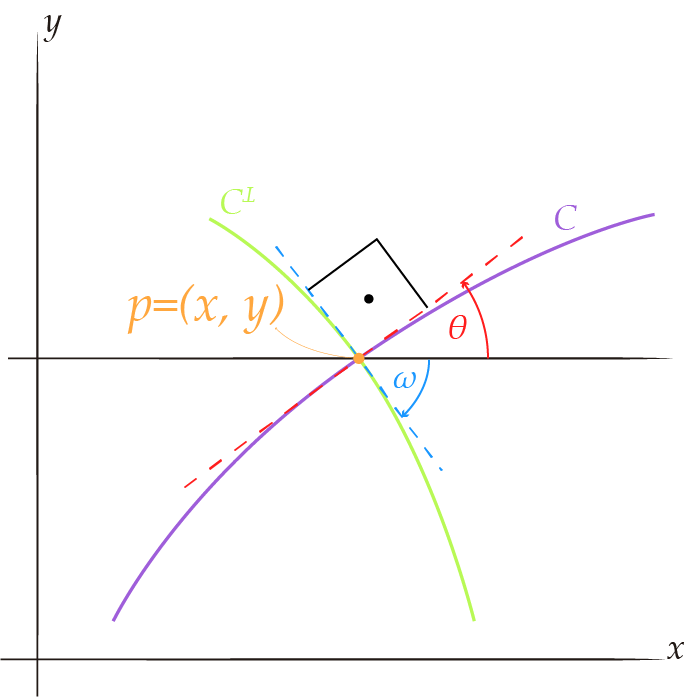
\includegraphics[width=0.48\textwidth]{1-trayectoriasortogonales.png}
  \end{center}
  \caption{Relaciones entre curvas ortogonales}\label{img:1-trayort}
\end{wrapfigure}
De la figura \ref{img:1-trayort} vemos que la pendiente de $C$ es $pend_C = \tan(\theta)$. Asimismo, $pend_{C^{\perp}} = \tan(\omega)$ y $\omega = \theta - \sfrac{\pi}{2}$. A partir de aquí desarrollamos:
$$
    \tan(\omega)=\frac{\sin(\theta-\sfrac{\pi}{2})}{\cos(\theta-\sfrac{\pi}{2})} = \frac{-\cos(\theta)}{\sin(\theta)} = -\frac{1}{\tan(\theta)}
$$
y por tanto,
\begin{equation} \label{eq:pendientes}
    pend_C \cdot pend_{C^{\perp}} = -1
\end{equation}

Nuestro objetivo es que dada una familia de curvas $fam_{C}$, podamos encontrar una (\textit{familia de}) curva que sea ortogonal a todas las de la familia en los puntos de cruce.\\\\
Supongamos que la familia original satisface una ecuación diferencial ordinaria $\mbf{y_1'} = f(x, \mbf{y_1})$. Queremos encontrar otra ecuación que defina a la ortogonal.\\\\
Como $fam_{C}$ sigue una EDO (\textit{ecuacion diferencial ordinaria}), podemos afirmar que $pend_{C} = \mbf{y_1'} = f(x, \mbf{y_1})$. Usando \ref{eq:pendientes}, $pend_{C^\perp} = \frac{-1}{f(x, \mbf{y_1})}$. Pero además, si $C^\perp$ sigue una EDO, está dada por una función $\mbf{y_2} = y_2(x)$ y entonces $\mbf{y_2'} = \frac{-1}{f(x, \mbf{y_1})}$.\\
Concluimos con que dada $fam_C$ descrita por $\mbf{y'}=f(x,\mbf{y})$, podemos encontrar $fam_{C^\perp}$ que satisface:
$$
    \mbf{y'} = -\frac{1}{f(x, \mbf{y})}
$$
\begin{eg}[Familia ortogonal a otra dada]
    Consideramos la familia: $x^2-\mbf{y}^2 = c \mid c \neq 0$\\
    Para cada $c$, eso define $\mbf{y}$ implícitamente en función de $x$.
    \begin{center}
        \vspace{1mm}
        \hfill
        \begin{tikzpicture}
            \begin{axis}[domain=-5:5,samples=150,
            restrict y to domain=-5:5,
            xtick=\empty,ytick=\empty,
            %extra x ticks={0.8,1.4}, linea vertical
            %extra y ticks=3.333333,extra y tick labels={$\frac{10}{3}$}, linea horizontal
            grid=both,axis lines=middle, axis equal
            ]
                \addplot+[no marks, thick, red, solid] ({x},{x}) node[pos=0.1, below, sloped] {$c=0$};
                \addplot+[no marks, thick, red, solid] ({x},{-x});
                %%%%%%%%%%%%%%%%%%%%%%%%%%%%%%%%%%%%%%%%%%%%%%%%%%%%%%%%%%%%%%%%%%%
                \addplot+[no marks, thick, coolblack, solid] ({(x^2+1)^(1/2)},{x}) node[pos=0.5, right] {$c > 0$};
                \addplot+[no marks, thick, coolblack, solid] ({-(x^2+1)^(1/2)},{x});
                \addplot+[no marks, thick, coolblack, densely dashed] ({(x^2+4)^(1/2)},{x});
                \addplot+[no marks, thick, coolblack, densely dashed] ({-(x^2+4)^(1/2)},{x});
                \addplot+[no marks, thick, coolblack, densely dotted] ({(x^2+9)^(1/2)},{x});
                \addplot+[no marks, thick, coolblack, densely dotted] ({-(x^2+9)^(1/2)},{x});
                %%%%%%%%%%%%%%%%%%%%%%%%%%%%%%%%%%%%%%%%%%%%%%%%%%%%%%%%%%%%%%%%%%%
                \addplot+[no marks, thick, black, solid] {(x^2+1)^(1/2)} node[pos=0.5, above, sloped] {$c < 0$};
                \addplot+[no marks, thick, black, solid] {-(x^2+1)^(1/2)};
                \addplot+[no marks, thick, black, densely dashed] {(x^2+4)^(1/2)};
                \addplot+[no marks, thick, black, densely dashed] {-(x^2+4)^(1/2)};
                \addplot+[no marks, thick, black, densely dotted] {(x^2+9)^(1/2)};
                \addplot+[no marks, thick, black, densely dotted] {-(x^2+9)^(1/2)};
            \end{axis}
        \end{tikzpicture}\hfill \break
        \vspace{1pt}
        $x^2-y^2=c$ para distintos valores de $c$.\\
        (También puede verse como las curvas de nivel del paraboloide hiperbólico)
    \end{center}
    \vspace{5pt}
    Para hallar la familia de curvas ortogonales vamos a seguir una serie de pasos:
    \begin{enumerate}
        \item \texttt{Encontrar una EDO que cumplan esas curvas.}\\
            $$
                x^2-\mbf{y}^2 = c \rightarrow \Dd{x} (x^2-y^2=c) \rightarrow 2x - 2\mbf{y}\mbf{y'} = 0 \implies \mbf{y'} = \frac{x}{\mbf{y}} = f(x,\mbf{y})
            $$
        \item \texttt{Econtrar la EDO para trayectorias ortogonales.}\\
            $$
                \mbf{y'} = -\frac{1}{f(x, \mbf{y})} = -\frac{\mbf{y}}{x}
            $$
        \item \texttt{Resolver la ecuación anterior}\\
            $$
                \dd{y}{x} = -\frac{\mbf{y}}{x} \implies -\frac{\mathrm{d}y}{\mbf{y}} = \frac{\mathrm{d}x}{x} \implies \log|y| = \log|x| + \mathcal{C}
            $$
            es decir,
            $$
                |\mbf{y}| = \frac{e^\mathcal{C}}{|x|} \implies |x\mbf{y}| = e^\mathcal{C} \implies x\mbf{y} = k : k = e^\mathcal{C} \lor k = e^{-\mathcal{C}} \implies \mbf{y} = \frac{k}{x}
            $$
    \end{enumerate}
    Con la solución general podemos representar parte de la familia:
    \begin{center}
        \vspace{1mm}
        \hfill
        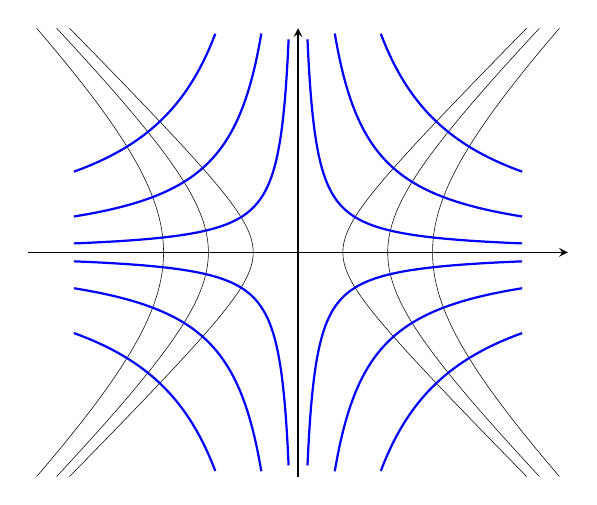
\begin{tikzpicture}
            \begin{axis}[domain=-5:5,samples=150,
            restrict y to domain=-5:5,
            xtick=\empty,ytick=\empty,
            %extra x ticks={0.8,1.4}, linea vertical
            %extra y ticks=3.333333,extra y tick labels={$\frac{10}{3}$}, linea horizontal
            grid=both,axis lines=middle, axis equal
            ]
                \addplot+[no marks, very thin, black, solid] ({(x^2+1)^(1/2)},{x});
                \addplot+[no marks, very thin, black, solid] ({-(x^2+1)^(1/2)},{x});
                \addplot+[no marks, very thin, black, solid] ({(x^2+4)^(1/2)},{x});
                \addplot+[no marks, very thin, black, solid] ({-(x^2+4)^(1/2)},{x});
                \addplot+[no marks, very thin, black, solid] ({(x^2+9)^(1/2)},{x});
                \addplot+[no marks, very thin, black, solid] ({-(x^2+9)^(1/2)},{x});
                %%%%%%%%%%%%%%%%%%%%%%%%%%%%%%%%%%%%%%%%%%%%%%%%%%%%%%%%%%%%%%%%%%%
                \addplot+[no marks, thick, blue, solid, samples=500] {1/x};
                \addplot+[no marks, thick, blue, solid, samples=500] {-1/x};
                \addplot+[no marks, thick, blue, solid, samples=300] {4/x};
                \addplot+[no marks, thick, blue, solid, samples=300] {-4/x};
                \addplot+[no marks, thick, blue, solid] {9/x};
                \addplot+[no marks, thick, blue, solid] {-9/x};
            \end{axis}
        \end{tikzpicture}\hfill \break
        \vspace{1pt}
        En azul posibles soluciones para disintos valores de $k$, en negro la familia original\\
        Se observa que son curvas ortogonales a la familia original.
    \end{center}
\end{eg}
